\documentclass{standalone}

\usepackage{tikz,pgf,pgfplots,circuitikz}
\pgfplotsset{compat=1.15}
\usetikzlibrary{intersections,arrows.meta,angles,calc,3d,decorations.pathmorphing}

\usepackage{amssymb,amsfonts,amsthm,mathtools}
\usepackage{physics,braket,bm}

\begin{document}  
  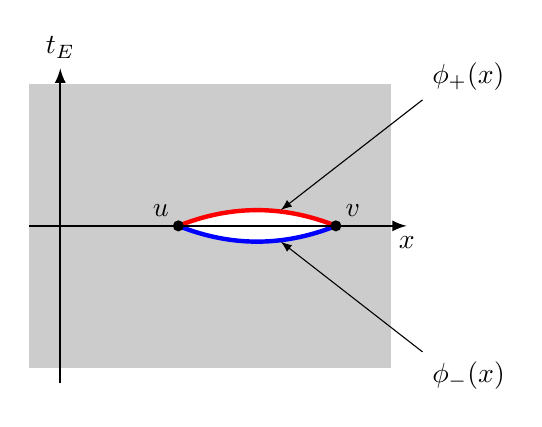
\begin{tikzpicture}
    \fill[opacity=0.2] (-0.4,1.8)--(4.2,1.8)--(4.2,-1.8)--(-0.4,-1.8);
    \fill[white] plot [smooth,samples=100,domain=1.5:3.5] (\x,{-0.2*(\x-2.5)*(\x-2.5)+0.2});
    \fill[white] plot [smooth,samples=100,domain=1.5:3.5] (\x,{0.2*(\x-2.5)*(\x-2.5)-0.2});
    
    \draw[red,ultra thick] plot [smooth,samples=100,domain=1.5:3.5] (\x,{-0.2*(\x-2.5)*(\x-2.5)+0.2});
    \draw[blue,ultra thick] plot [smooth,samples=100,domain=1.5:3.5] (\x,{0.2*(\x-2.5)*(\x-2.5)-0.2});

    \draw[-latex](4.6,1.6)--(2.8,0.2);
    \draw (4.6,1.6) node[above right]{$\phi_+(x)$};
    \draw[-latex](4.6,-1.6)--(2.8,-0.2);
    \draw (4.6,-1.6) node[below right]{$\phi_-(x)$};

    \draw[-latex,thick] (-0.4,0)--(4.4,0) node [below]{$x$};
    \draw[-latex,thick] (0,-2.0)--(0,2.0) node [above] {$t_E$};
    \fill[black] (1.5,0) circle (2pt) node [above left]{$u$};
    \fill[black] (3.5,0) circle (2pt) node [above right]{$v$};
  \end{tikzpicture}
\end{document}
